
\documentclass[12pt]{article}
\usepackage{setspace}   % paquete para interlineado
\usepackage{newtxtext,newtxmath} % Times New Roman

%otra opcion para times roman adaptable a versiones
%\usepackage{mathptmx}

%haber si funciona mas parecido a word
\setstretch{1.5}  
%\usepackage[protrusion,expansion]{microtype}
%\onehalfspacing               % interlineado 1.5
\usepackage{amsmath} % Para usar \text{}
\usepackage[utf8]{inputenc}
\usepackage[spanish]{babel}
\usepackage[letterpaper, left=3cm, right=2.5cm, top=2.5cm, bottom=2.5cm]{geometry}
\usepackage{graphicx}
\usepackage{titlesec}
\usepackage{setspace}
\usepackage{lipsum}
\geometry{margin=1in}


%PAQUETE para incluir PDF´s
\usepackage{pdfpages} % para incluir PDFs

%------PAQUETE PARA INDICE--------
% ==== Estilo del Índice (como en tu imagen) ====
\usepackage{xcolor}
\usepackage{tocloft}
\usepackage{hyperref}
\hypersetup{colorlinks=true, linkcolor=black}


% --- Título del índice ---
\renewcommand{\contentsname}{Índice}
\renewcommand{\cfttoctitlefont}{\Huge\bfseries\color{black}}
\renewcommand{\cftaftertoctitle}{\par\vskip 0.5em}

% --- Secciones sin numeración ---
\setcounter{secnumdepth}{0}   % oculta numeración de secciones

% --- Líneas punteadas (dot leaders) ---
\renewcommand{\cftsecleader}{\cftdotfill{\cftdotsep}}

\renewcommand{\cftsecfont}{\bfseries\color{black}}       % sección en negrita
\renewcommand{\cftsecpagefont}{\bfseries\color{black}}   % número en negrita
\setlength{\cftbeforesecskip}{6pt}          % espaciado
\setlength{\cftbeforesubsecskip}{3pt}
\setlength{\cftbeforesubsubsecskip}{2pt}
\setcounter{tocdepth}{3}                     % profundidad del índice





\begin{document}
	%-----------------CARATULA-------------
	
\includepdf{portadaU2/caratulaU}
	
	% ====== ÍNDICE ======
	\tableofcontents
	\newpage
	
	% Hoja Adjunta (entra al índice sin título en página aparte)
	
\includepdf[  pages=-,
	pagecommand={},  % sin encabezado extra
	addtotoc={1,section,1,{Hoja Adjunta},sec:hoja}
	]{hoja/hojaadjunta}
	
	
	
	
	%-------------OFICIO FIRMADO---------------
	
\includepdf[
	pages=-,            % o pages=- para todas
	fitpaper=false,     % no adaptar la hoja al PDF
	scale=0.85,         % reduce el contenido
	offset=0mm 0mm,     % mueve (x,y). Ej: 0mm -5mm para bajar un poco
	pagecommand={\thispagestyle{plain}}, % (opcional) número de página visible
	 addtotoc={1,section,1,{Oficio Firmado},sec:oficio}
	]{scaner/oficiofirmado}
	
	%------------RESPUESTA INSTITUCIÓN---------------------
	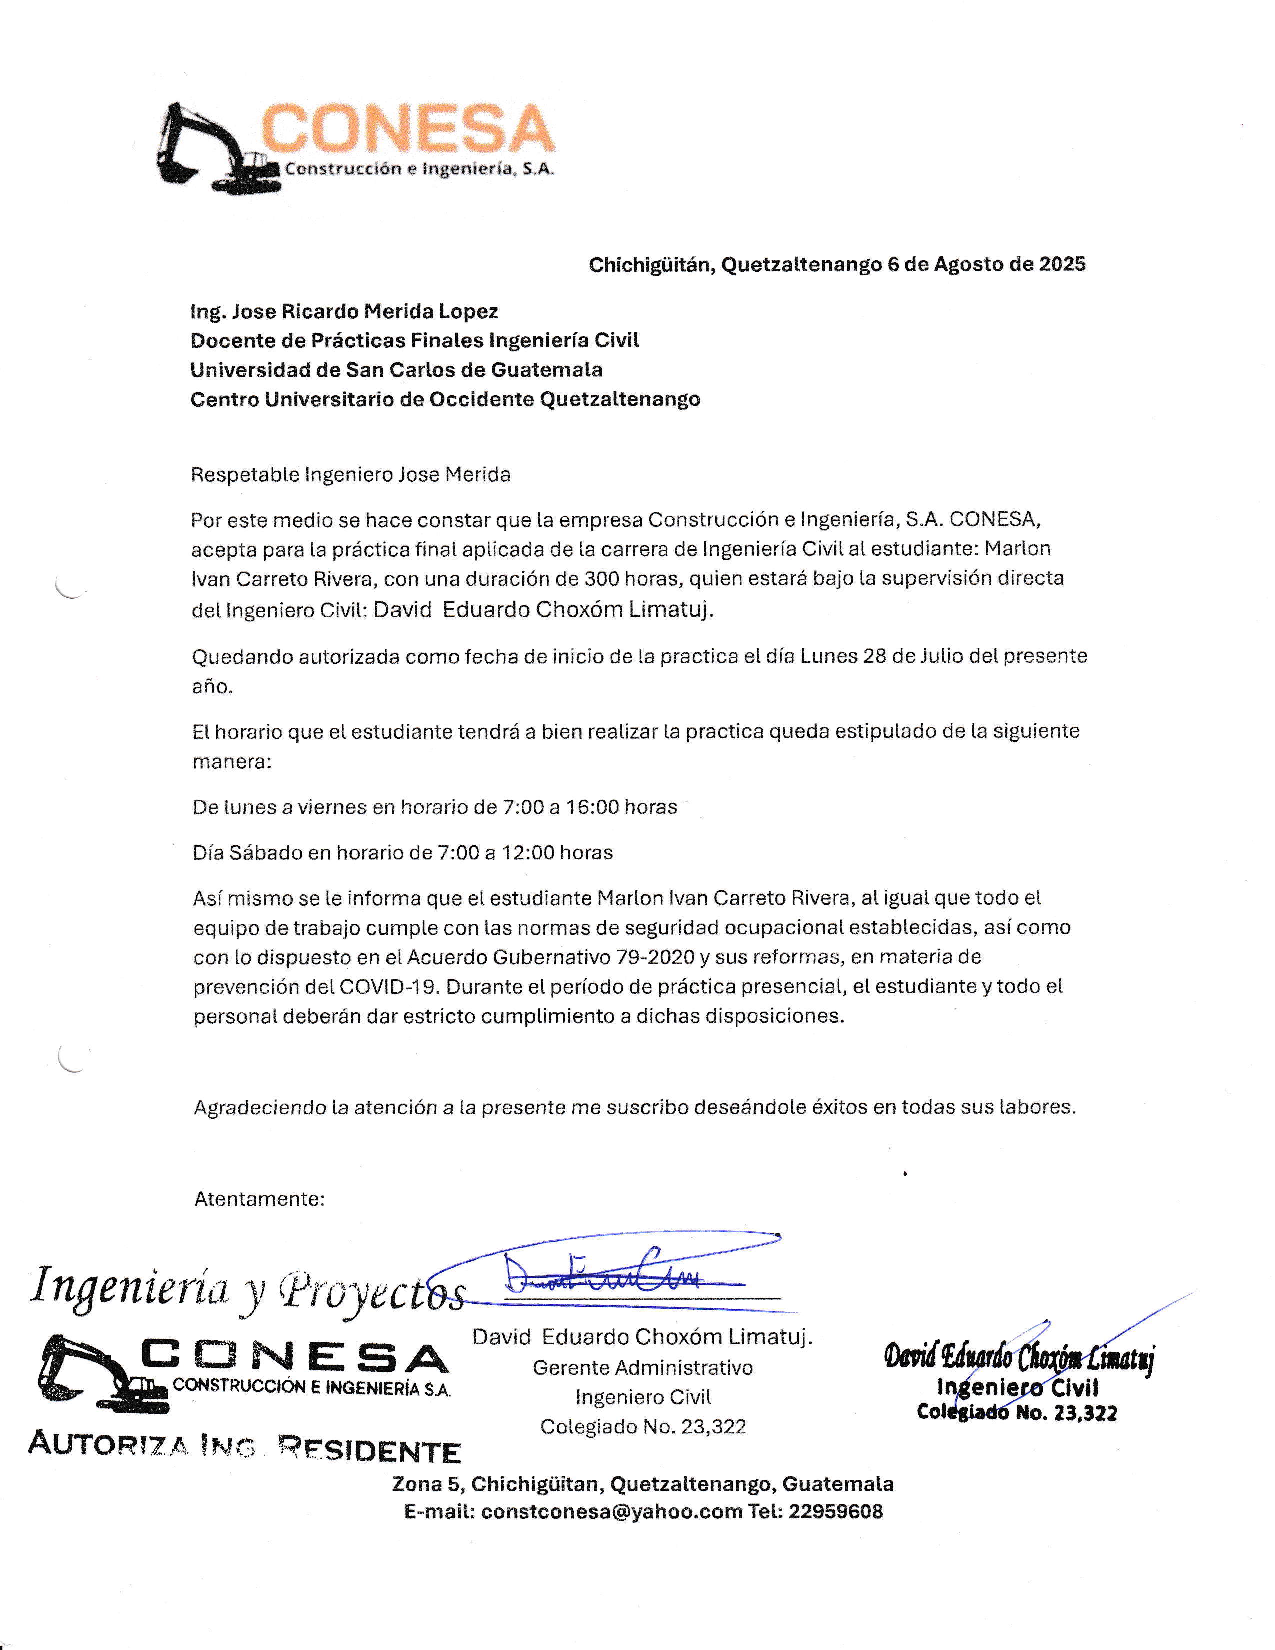
\includepdf[
	pages=-,            % o pages=- para todas
	fitpaper=false,     % no adaptar la hoja al PDF
	scale=0.85,         % reduce el contenido
	offset=0mm 0mm,     % mueve (x,y). Ej: 0mm -5mm para bajar un poco
	pagecommand={\thispagestyle{plain}}, % (opcional) número de página visible
	 addtotoc={1,section,1,{Respuesta Institución},sec:conesa}
	]{scaner/respuestaconesa}
	
	%------------BITACORA---------------------
	
\includepdf[pages=-,
	pagecommand={\thispagestyle{plain}}, % (opcional) número de página visible
	addtotoc={1,section,1,{Bitacora},sec:Bitacora}
	 ]{bitacora/bitacora}
	
	
	
	
	
	
	%----------------INVESTIGACION---------------	
	
	
\includepdf[pages=-,pagecommand={},
	 addtotoc={1,section,1,{Investigación},sec:investigacion}
	]{investigacion/investigacion}
	
	
\end{document}